\documentclass{standalone}

\usepackage{tikz}
\usetikzlibrary{fit, shapes}

\begin{document}
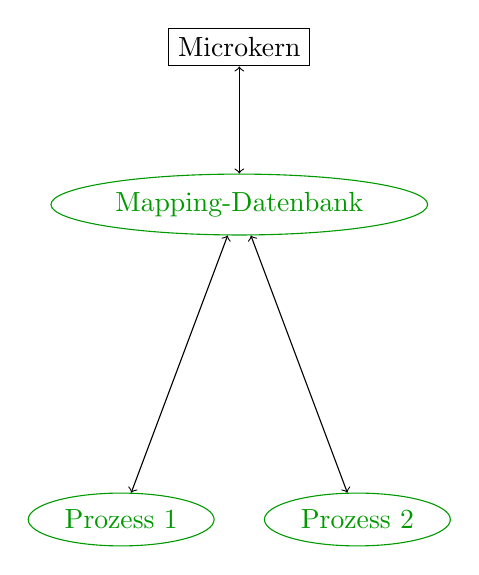
\begin{tikzpicture} [
  y=1mm,
  x=1mm,
  task/.style={draw=green!60!black, text=green!60!black, ellipse}
  ]
  \node(task1)[task, at={(0,0)}]{Prozess 1};
  \node(task2)[task, at={(30,0)}]{Prozess 2};
  \node(map-db)[task, at={(15,40)}]{Mapping-Datenbank};
  \node(kern)[rectangle, draw, at={(15,60)}]{Microkern};
  
  \draw[<->] (task1) -- (map-db);
  \draw[<->] (task2) -- (map-db);
  \draw[<->] (map-db) -- (kern);
\end{tikzpicture}
\end{document}